\documentclass[]{article}

%opening

\usepackage{amsmath}
\usepackage{amsfonts}
\usepackage{float}
\usepackage{hyperref}
\usepackage[explicit]{titlesec}
\usepackage{xcolor}
\usepackage{graphicx}

\title{Progress Report 1}
\author{Jayveersinh Raj, Makar Shevchenko, Nikolay Pavlenko}
\date{March 7th, 2023}

\begin{document}
	
	\maketitle
	
	\section{Current Progress}
	
	\subsection{Research}
	
	\subsubsection{Primary NLP Topics}
	
	Before moving forward with the project, we had to map out some important NLP-relevant topics we would be trying to cover while building this model. After discussing them, we have accepted \textbf{Sentiment Analysis} to be the primary NLP technique we will be implementing in our model. To narrow down the task, we have chosen the implementation of \textbf{Toxic Comment Classification} as our current goal. Hopefully, in the future we will also be able to implement \textbf{Machine Translation} from English into Romanian, thereby demonstrating that our model can work on more than one language effectively. \\
	
	\subsubsection{Datasets Exploration}
	
	After setting our goals as described above, we started searching for various datasets that would allow us to develop the model. In the end, three most relevant datasets were found:
	\begin{enumerate}
		\item Personal attacks dataset from Wikipedia's Detox project\cite{wikiDetox},
		\item Jigsaw and Google toxic comment analysis dataset\cite{jigsaw},
		\item IMDB ratings sentiment dataset\cite{imdb}.
	\end{enumerate}

	\subsubsection{Results}
	
	To jump-start our project, we have begun working with the Jigsaw dataset first. It was chosen over the other 2 datasets, as it is more vivid than the competition, and its classification of toxicity into several levels is very useful in the particular problem we are trying to solve. This dataset is also high-quality and easy to clean, so it makes for a good starting point from where we can get some results from the model.
	
	\subsection{Data Understanding}
	
	\subsubsection{Initial Data Collection}
	
	In order for a dataset to be relevant in a Sentiment Analysis task (and specifically in our case of toxic comment classification), it has to fulfill certain conditions:
	\begin{enumerate}
		\item It must contain text data of messages that are to be classified.
		\item It must contain labeled data, that would attach a specific level of toxicity to each message.
		\item It has to be large enough for the model to be able to train effectively.
		\item The dataset has to be diverse enough for the developed model to generalize better.
		\item The dataset should ideally be high-quality, devoid of noise, missing data and having balanced labels across different classes.
	\end{enumerate}
	We have used all those conditions as guidelines while searching for datasets for our model and performing data preprocessing.
	
	\subsubsection{Data Description}
	
	Dataset chosen for initial development of our model contained the following features:
	\begin{figure}[h]
		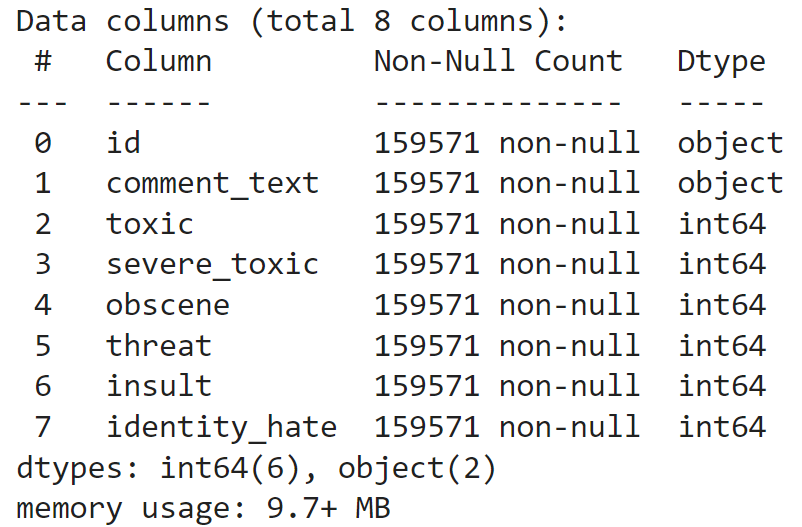
\includegraphics{screenshot1.png}
	\end{figure}\\
	\textbf{comment\_text} column is the one we will be using to develop the toxicity classification, while columns from \textbf{toxic} to \textbf{identity\_hate} are binary non-exclusive labels describing various toxicity levels present in the comments.
	
	\subsubsection{Data Exploration}
	
	In order to explore our dataset, we have gathered important statistical characteristics of all the labels in it, and plotted graphs and a heatmap that highlight class imbalances and correlations between different features:
	\begin{figure}[h]
		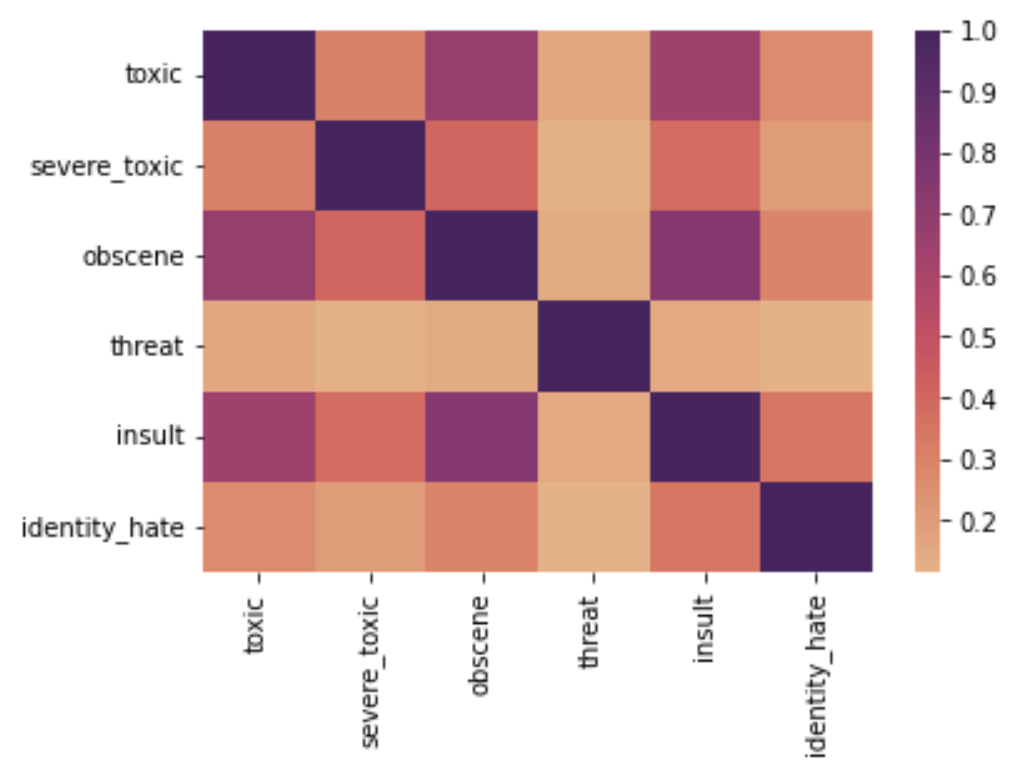
\includegraphics{screenshot2.png}
	\end{figure}\\
	
	\subsubsection{Verification of Data Quality}
	
	In order to make sure that the dataset is of a relatively high quality, we have checked if it contained any null values - thankfully, it did not: 
	\begin{figure}[h]
		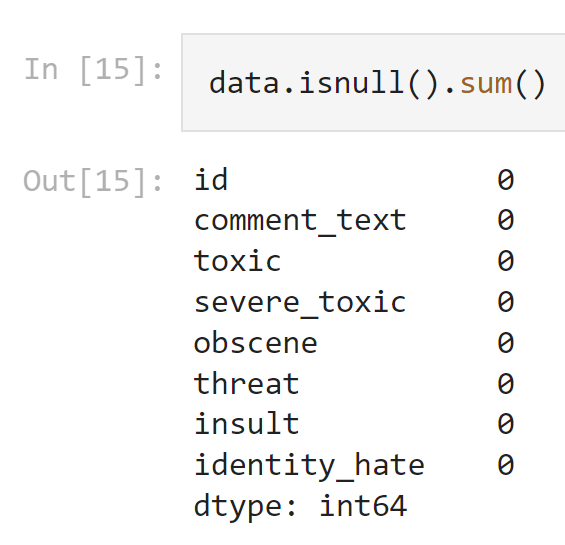
\includegraphics[scale=0.9]{screenshot3.png}
	\end{figure}\\
	
	\subsection{Data Preprocessing}
	
	During data preprocessing a few important changes were introduced to the dataset:
	\begin{enumerate}
		\item \textbf{id} column was dropped, as it was irrelevant in the task our model is set to achieve.
		\item Due to extremely sparse nature of the binary labels in the dataset, we have decided to merge them into a single true/false column, that is supposed to represent any level of toxicity found in a comment. It is a temporary measure, and the initial dataset with multiple toxicity labels was preserved for future work.
		\item Since various features were found to be heavily imbalanced during data exploration, data was resampled to allow for the same number of toxic and non-toxic comments in the dataset.
	\end{enumerate}

	\subsection{Modeling}
	
	\subsubsection{Architecture}
	
	In order to be able to classify the comments according to their toxicity level, we first have to encode the text data. We use the pre-trained \textbf{BERT encoder} for that purpose, transforming the text to classifiable tensors. \\
	
	The initial attempt at classification was done with the help of \textbf{Support Vector Machine(SVM)}, implementation taken from sklearn library. However, it failed due to extremely long inference time of the model - from 15 to 35 seconds per sample, which is far too long considering the large size of our dataset.\\
	
	For that reason we have decided to avoid SVM and instead focused on \textbf{XLM-R-Classifier}, which is supposed to work well on multilingual data - that makes it very relevant for the particular conditions of our project.
	
	\subsubsection{Hardware}
	
	Currently we have trained our model using Google Colab, as it provides a decent platform to start developing our model on, though we are considering options on improving available hardware resources in the future.
	
	\subsection{Evaluation}
	
	As mentioned prior, no results have been achieved with the help of the BERT encoder + SVM classifier, with BERT working extremely slowly on Google Colab, taking 3 seconds per sample. \\
	On the other hand, XLM-Roberta embedder used in conjunction with XLM-Roberta classifier led to very good results. It worked well on several Indo-European languages: English, Hindi, French, etc., and reached an F1-score of 0.96 in particular on the english dataset, using a 90-10 training/validation split.
	
	\section{Team Member Contribution}
	
	\begin{itemize}
		\item \textbf{Jayveersinh Raj}: datasets exploration, development and evaluation of XLM-Roberta embedder-classifier pipeline;
		\item \textbf{Makar Shevchenko}: data understanding and preprocessing, development of BERT encoder - SVM classifier pipeline, organizational responsibilities;
		\item \textbf{Nikolay Pavlenko}: progress evaluation, composition of intermediary report. 
	\end{itemize}

	\section{Plan for the Next Three Weeks}
	
	Considering the results achieved during the previous weeks, we have decided to continue the development of the XML-Roberta embedder + XLM-Roberta classifier, while pausing and reevaluating the BERT-SVM pipeline until better hardware resources could be obtained. Until then, some other pipeline could be developed using other classifiers from sklearn library. \\
	We will further seek to collect more data to augment the existing selection, particularly focusing on non-English datasets, so we would have the possibility of testing zero-shot cross-lingual transfer.
	
	\section{Github Link}
	\textbf{Notice:} The repository is private, so if you want to check the current state of the project, please write to \href{https://t.me/syrexminus}{\emph{Makar Shevchenko}} on Telegram to get access to it.
	\textbf{Link:}\href{https://github.com/SyrexMinus/cross\_lingual\_nlp}{\emph{https://github.com/SyrexMinus/cross\_lingual\_nlp}}
	
	\begin{thebibliography}{9}
		\bibitem{wikiDetox} https://figshare.com/articles/dataset/Wikipedia\_Talk\_Labels\_Personal\_Attacks/4054689
		\bibitem{jigsaw}
		https://www.kaggle.com/competitions/jigsaw-toxic-comment-classification-challenge/data
		\bibitem{imdb}
		https://ai.stanford.edu/~amaas/data/sentiment/
	\end{thebibliography}
	
\end{document}
